\documentclass[12pt,a4paper]{article}
\usepackage[utf8]{vietnam}
\usepackage{amsmath,amssymb}
\usepackage{geometry}
\geometry{top=1.5cm,bottom=1.2cm,left=1.4cm,right=1.4cm,headheight=28pt,headsep=12pt,footskip=18pt}
\usepackage{tikz}
\usepackage{xcolor}
\usepackage{enumerate}
\usepackage{graphicx}
\usepackage[version=4]{mhchem}
\usepackage{fancyhdr}
\usepackage{ex_test}

\renewcommand{\baselinestretch}{1.0}
\setlength{\parskip}{1pt}

\definecolor{hfRed}{RGB}{211,47,47}
\definecolor{hfGreen}{RGB}{139,195,144}

\pagestyle{fancy}
\fancyhf{}
\fancyhead[L]{\small\itshape\color{hfRed} Tài liệu lưu hành nội bộ}
\fancyhead[R]{\small\itshape\color{hfRed} Thầy \textbf{TRẦN VĂN THẠNH} - 0777.470.803}
\renewcommand{\headrulewidth}{0.8pt}
\renewcommand{\headrule}{\hbox to\headwidth{\color{hfGreen}\leaders\hrule height \headrulewidth\hfill}}

\fancyfoot[L]{\small\itshape\color{hfRed} CS1: 6/15 Nguyễn Hoàng, P. Kim Long, TP Huế \quad|\quad CS2: 24 Đặng Thái Thân, TP Huế}
\fancyfoot[R]{\small\bfseries\color{hfRed} Trang \thepage}
\renewcommand{\footrulewidth}{0.8pt}
\renewcommand{\footrule}{\hbox to\headwidth{\color{hfGreen}\leaders\hrule height \footrulewidth\hfill}}

\fancypagestyle{firstpage}{
  \fancyhf{}
  \renewcommand{\headrulewidth}{0pt}
  \fancyfoot[L]{\small\itshape\color{hfRed} CS1: 6/15 Nguyễn Hoàng, P. Kim Long, TP Huế \quad|\quad CS2: 24 Đặng Thái Thân, TP Huế}
  \fancyfoot[R]{\small\bfseries\color{hfRed} Trang \thepage}
  \renewcommand{\footrulewidth}{0.8pt}
  \renewcommand{\footrule}{\hbox to\headwidth{\color{hfGreen}\leaders\hrule height \footrulewidth\hfill}}
}

\begin{document}
\thispagestyle{firstpage}

\noindent
\begin{minipage}[t]{0.45\textwidth}
	\centering\fontsize{10pt}{12pt}\selectfont
	\textbf{SỞ GIÁO DỤC VÀ ĐÀO TẠO TP. HUẾ}\\
	\textbf{TRƯỜNG THPT NGUYỄN CHÍ THANH}\\
	\textbf{ĐỀ CHÍNH THỨC}\\
	\textit{(Đề thi có 03 trang)}
\end{minipage}\hfill
\begin{minipage}[t]{0.53\textwidth}
	\centering\small
	\textbf{ĐỀ KIỂM TRA GIỮA HỌC KỲ I -- NĂM HỌC 2025 - 2026}\\
	\textbf{MÔN: HOÁ HỌC. Lớp 11}\\
	\textit{Thời gian làm bài: 45 phút (không kể thời gian phát đề)}\\
	\fbox{\textbf{MÃ ĐỀ: 104}}
\end{minipage}

\smallskip
\begin{center}
	{\color{hfRed}\textbf{\large (BẢN GIÁO VIÊN -- CÓ LỜI GIẢI CHI TIẾT)}}
\end{center}

\smallskip
\noindent\hrulefill
\smallskip

\noindent\textbf{Họ, tên thí sinh:} \dotfill\ \textbf{Lớp:} \dotfill\ \textbf{Số báo danh:} \dotfill

\smallskip
\noindent\textit{(Cho biết nguyên tử khối: H = 1; C = 12; N = 14; O = 16; Na = 23; S = 32; Cl = 35,5; Ba = 137; Al = 27; Cu = 64; Fe = 56).}
\smallskip

\noindent
\textbf{PHẦN I. Câu trắc nghiệm nhiều phương án lựa chọn: (16 câu -- 4 điểm)}\\
\textit{Thí sinh trả lời từ câu 1 đến câu 16. Mỗi câu thí sinh chỉ chọn một phương án.}

\Opensolutionfile{ans}[ans-hoa11-ma104gv]

\begin{ex}
Các dung dịch sau đây có cùng nồng độ 1M, dd nào dẫn điện tốt nhất?
\choice
{$\ce{Ba(OH)2}$}
{\True $\ce{Al2(SO4)3}$}
{$\ce{H2SO4}$}
{$\ce{NH4NO3}$}
\loigiai{
Khả năng dẫn điện của dung dịch phụ thuộc vào tổng nồng độ các ion trong dung dịch:\\
- $\ce{Ba(OH)2 -> Ba^{2+} + 2OH-} \implies$ tổng nồng độ ion $= 3\text{ M}$.\\
- $\ce{Al2(SO4)3 -> 2Al^{3+} + 3SO4^{2-}} \implies$ tổng nồng độ ion $= 5\text{ M}$.\\
- $\ce{H2SO4 -> 2H+ + SO4^{2-}} \implies$ tổng nồng độ ion $= 3\text{ M}$.\\
- $\ce{NH4NO3 -> NH4+ + NO3-} \implies$ tổng nồng độ ion $= 2\text{ M}$.\\
Do đó dung dịch $\ce{Al2(SO4)3}$ có nồng độ ion lớn nhất nên dẫn điện tốt nhất.\\
\textbf{Chọn B.}}
\end{ex}

\begin{ex}
Khí thải công nghiệp, khí thải động cơ (ô tô, xe máy ...) là nguyên nhân chủ yếu gây mưa acid. Dãy nào dưới đây gồm các chất có trong các loại khí thải này và là nguyên nhân trực tiếp gây mưa acid?
\choice
{$\ce{SO2}, \ce{CO}, \ce{NO}$.}
{$\ce{NO2}, \ce{CO2}, \ce{CO}$.}
{\True $\ce{NO}, \ce{NO2}, \ce{SO2}$.}
{$\ce{SO2}, \ce{CO}, \ce{NO2}$.}
\loigiai{
Mưa acid được hình thành chủ yếu do các oxide của nitrogen ($\ce{NO}, \ce{NO2}$) và sulfur dioxide ($\ce{SO2}$) khi phản ứng với oxygen và hơi nước trong khí quyển tạo thành $\ce{HNO3}$ và $\ce{H2SO4}$. Khí $\ce{CO}$ không gây mưa acid.\\
\textbf{Chọn C.}}
\end{ex}

\begin{ex}
Cho các phản ứng sau:\\
(1) $\ce{N2 + O2 ->[t^\circ, xt] 2NO}$;\\
(2) $\ce{N2 + 3H2 <=>[t^\circ, xt] 2NH3}$.\\
Trong hai phản ứng trên thì nitrogen
\choice
{\True thể hiện tính khử và tính oxi hóa.}
{không thể hiện tính khử và tính oxi hóa.}
{chỉ thể hiện tính oxi hóa.}
{chỉ thể hiện tính khử.}
\loigiai{
- Trong (1): $\overset{0}{\ce{N}}_2 \to 2\overset{+2}{\ce{N}}\ce{O}$, số oxi hóa tăng nên $\ce{N2}$ là chất khử.\\
- Trong (2): $\overset{0}{\ce{N}}_2 \to 2\overset{-3}{\ce{N}}\ce{H3}$, số oxi hóa giảm nên $\ce{N2}$ là chất oxi hóa.\\
Vậy nitrogen thể hiện tính khử và tính oxi hóa.\\
\textbf{Chọn A.}}
\end{ex}

\begin{ex}
Nhận xét nào sau đây \textbf{không đúng}?
\choice
{\True Phản ứng một chiều là phản ứng luôn xảy ra không hoàn toàn.}
{Trong phản ứng thuận nghịch, các chất sản phẩm có thể phản ứng với nhau để tạo thành chất đầu.}
{Trong phản ứng một chiều, các chất sản phẩm không phản ứng được với nhau tạo thành chất đầu.}
{Phản ứng thuận nghịch là phản ứng xảy ra theo hai chiều trái ngược nhau trong cùng điều kiện.}
\loigiai{
Phản ứng một chiều là phản ứng xảy ra hoàn toàn (kết thúc phản ứng thì chất phản ứng hết). Nhận xét A là không đúng.\\
\textbf{Chọn A.}}
\end{ex}

\begin{ex}
Trong y học, vì sao nitrogen lỏng được dùng để bảo quản mẫu vật?
\choice
{\True Do nitrogen hóa lỏng ở nhiệt độ thấp.}
{Do nitrogen không duy trì sự hô hấp.}
{Do nitrogen tan ít rất trong nước.}
{Do nitrogen là chất khí không màu, không mùi, không vị.}
\loigiai{
Nitrogen hóa lỏng ở nhiệt độ rất thấp ($-196^\circ\text{C}$), tạo môi trường nhiệt độ siêu thấp làm ngừng mọi hoạt động trao đổi chất và vi sinh vật để bảo quản mẫu vật lâu dài mà không bị biến tính.\\
\textbf{Chọn A.}}
\end{ex}

\begin{ex}
Chất nào sau đây là chất điện li?
\choice
{Glucose.}
{Saccharose.}
{\True Sodium hydroxide.}
{Alcohol ethylic.}
\loigiai{
Sodium hydroxide ($\ce{NaOH}$) là một base mạnh, tan hoàn toàn trong nước và phân li ra ion $\ce{Na+}$ và $\ce{OH-}$ nên là chất điện li.\\
\textbf{Chọn C.}}
\end{ex}

\begin{ex}
Cho $m$ gam Na vào nước dư thu được $1{,}5\text{ L}$ dung dịch có $\text{pH} = 12$. Giá trị của $m$ là
\choice
{$0{,}23\text{ gam}$.}
{$0{,}46\text{ gam}$.}
{$0{,}115\text{ gam}$.}
{\True $0{,}345\text{ gam}$.}
\loigiai{
$\text{pH} = 12 \implies \text{pOH} = 2 \implies [\ce{OH-}] = 0{,}01\text{ M}$.\\
Số mol $\ce{OH-}$ trong $1{,}5\text{ L}$ dung dịch: $n_{\ce{OH-}} = 0{,}01 \times 1{,}5 = 0{,}015\text{ mol}$.\\
Phương trình phản ứng: $\ce{Na + H2O -> NaOH + 1/2 H2 ^}$.\\
$n_{\ce{Na}} = n_{\ce{OH-}} = 0{,}015\text{ mol} \implies m = 0{,}015 \times 23 = 0{,}345\text{ gam}$.\\
\textbf{Chọn D.}}
\end{ex}

\begin{ex}
Chuẩn độ dung dịch $\ce{NaOH}$ chưa biết chính xác nồng độ (biết nồng độ trong khoảng gần với $0{,}1\text{ M}$) bằng dung dịch $\ce{HCl}\ 0{,}1\text{ M}$ với chỉ thị phenolphtalein. Chất đóng vai trò là dung dịch chuẩn là?
\choice
{Phenolphtalein.}
{$\ce{NaCl}$.}
{$\ce{NaOH}$.}
{\True $\ce{HCl}$.}
\loigiai{
Dung dịch chuẩn là dung dịch đã biết trước chính xác nồng độ. Ở đây $\ce{HCl}\ 0{,}1\text{ M}$ đóng vai trò là dung dịch chuẩn.\\
\textbf{Chọn D.}}
\end{ex}

\begin{ex}
Để hạn chế hiện tượng phú dưỡng, ta có thể dùng bao nhiêu biện pháp sau đây?\\
(1) Tạo điều kiện để nước trong kênh, rạch, ao, hồ được lưu thông.\\
(2) Xử lí nước thải trước khi chảy vào kênh rạch ao hồ.\\
(3) Sử dụng phân bón đúng lượng, đúng cách \& đúng thời điểm.
\choice
{1.}
{2.}
{0.}
{\True 3.}
\loigiai{
Cả 3 biện pháp đều góp phần quan trọng ngăn chặn và giảm thiểu hiện tượng phú dưỡng nguồn nước.\\
\textbf{Chọn D.}}
\end{ex}

\begin{ex}
Trong phản ứng tổng hợp $\ce{NH3}$ theo quá trình Haber hỗn hợp $\ce{N2}$ \& $\ce{H2}$ (tỉ lệ mol $x : y$) được nén ở áp suất cao và đưa vào tháp tổng hợp ammonia trong điều kiện nhiệt độ, áp suất và chất xúc tác thích hợp. Tỉ lệ mol $x : y$ là?
\choice
{$1 : 2$.}
{$2 : 1$.}
{\True $1 : 3$.}
{$3 : 1$.}
\loigiai{
Theo phương trình: $\ce{N2 + 3H2 <=> 2NH3}$, tỉ lệ mol hệ số tỉ lượng của hỗn hợp nạp vào tháp tổng hợp Haber là $n_{\ce{N2}} : n_{\ce{H2}} = 1 : 3$.\\
\textbf{Chọn C.}}
\end{ex}

\begin{ex}
Xét cân bằng:\\
(1) $\ce{H2(g) + I2(g) <=> 2HI(g)} \quad (K_1)$\\
(2) $\ce{2HI(g) <=> H2(g) + I2(g)} \quad (K_2)$\\
Mối quan hệ giữa $K_1$ và $K_2$ là:
\choice
{$K_1 = 2K_2$.}
{$K_1 = K_2$.}
{$K_1 = \sqrt{K_2}$.}
{\True $K_1 = K_2^{-1}$.}
\loigiai{
$K_1 = \frac{[\ce{HI}]^2}{[\ce{H2}][\ce{I2}]}$ và $K_2 = \frac{[\ce{H2}][\ce{I2}]}{[\ce{HI}]^2} \implies K_1 = \frac{1}{K_2} = K_2^{-1}$.\\
\textbf{Chọn D.}}
\end{ex}

\begin{ex}
Công thức Lewis của $\ce{NH3}$ là:
\begin{center}
	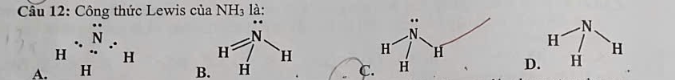
\includegraphics[width=0.6\textwidth]{images_crop/de104_cau12_lewis.png}
\end{center}
\choice
{Công thức A}
{Công thức B}
{\True Công thức C}
{Công thức D}
\loigiai{
Trong phân tử $\ce{NH3}$, nguyên tử N tạo 3 liên kết đơn với 3 nguyên tử H và còn lại 1 cặp electron tự do trên nguyên tử N. Do đó công thức C là công thức Lewis đúng.\\
\textbf{Chọn C.}}
\end{ex}

\begin{ex}
Kim loại không bị hòa tan trong dung dịch acid $\ce{HNO3}$ đặc nguội, nhưng tan được trong dung dịch $\ce{NaOH}$ là:
\choice
{$\ce{Mg}$}
{\True $\ce{Al}$}
{$\ce{Fe}$}
{$\ce{Pb}$}
\loigiai{
Nhôm ($\ce{Al}$) bị thụ động hóa trong $\ce{HNO3}$ đặc nguội (không tan), nhưng phản ứng mạnh với dung dịch kiềm $\ce{NaOH}$:\\
$\ce{2Al + 2NaOH + 6H2O -> 2Na[Al(OH)4] + 3H2 ^}$.\\
\textbf{Chọn B.}}
\end{ex}

\begin{ex}
Cân bằng hoá học là một trạng thái của phản ứng thuận nghịch tại đó:
\choice
{tốc độ phản ứng thuận bằng một nửa tốc độ phản ứng nghịch.}
{tốc độ phản ứng không thay đổi.}
{tốc độ phản ứng thuận bằng hai lần tốc độ phản ứng nghịch.}
{\True tốc độ phản ứng thuận bằng tốc độ phản ứng nghịch.}
\loigiai{
Cân bằng hóa học là trạng thái tại đó tốc độ phản ứng thuận bằng tốc độ phản ứng nghịch ($v_{\text{thuận}} = v_{\text{nghịch}}$).\\
\textbf{Chọn D.}}
\end{ex}

\begin{ex}
Tổng hệ số (các số nguyên, tối giản) của tất cả các chất trong phương trình phản ứng giữa Cu với dung dịch $\ce{HNO3}$ đặc là
\choice
{11.}
{9.}
{\True 10.}
{8.}
\loigiai{
Phương trình hóa học: $\ce{Cu + 4HNO3 -> Cu(NO3)2 + 2NO2 ^ + 2H2O}$.\\
Tổng hệ số tối giản: $1 + 4 + 1 + 2 + 2 = 10$.\\
\textbf{Chọn C.}}
\end{ex}

\begin{ex}
Có thể phân biệt muối ammonium với các muối khác bằng cách cho nó tác dụng với dung dịch kiềm đun nóng, vì
\choice
{thoát ra một chất khí màu nâu đỏ, làm xanh giấy quỳ tím ẩm.}
{thoát ra một chất khí màu lục nhạt.}
{thoát ra chất khí không màu, không mùi.}
{\True thoát ra một chất khí không màu, mùi khai, làm xanh giấy quỳ tím ẩm.}
\loigiai{
Đun nóng muối ammonium với kiềm: $\ce{NH4+ + OH- ->[t^\circ] NH3 ^ + H2O}$.\\
Khí $\ce{NH3}$ sinh ra không màu, mùi khai đặc trưng, làm xanh quỳ tím ẩm.\\
\textbf{Chọn D.}}
\end{ex}

\Closesolutionfile{ans}

\bigskip
\noindent
\textbf{PHẦN II. Câu trắc nghiệm đúng sai: (2 câu -- 2 điểm)}\\
\textit{Thí sinh trả lời từ câu 1 đến câu 2. Trong mỗi ý a), b), c), d) ở mỗi câu thí sinh chọn đúng hoặc sai.}

\begin{ex}
Hiện tượng phú dưỡng là một biểu hiện của môi trường ao, hồ bị ô nhiễm do dư thừa các chất dinh dưỡng.
\choiceTF
{\True a) Chất thải công nghiệp, chất thải sinh hoạt, ... khi không được xử lí theo quy chuẩn, nếu thải vào sông, hồ cũng gây ra hiện tượng phú dưỡng.}
{b) Thông thường, khi hàm lượng calcium trong nước đạt $300\ \mu\text{g/L}$ và hàm lượng magnesium đạt $20\ \mu\text{g/L}$ sẽ gây hiện tượng phú dưỡng.}
{\True c) Có thể quan sát được hiện tượng phú dưỡng thông qua sự xuất hiện dày đặc của tảo xanh trong nước.}
{\True d) Hiện tượng phú dưỡng gây cản trở hấp thụ ánh sáng mặt trời vào nước, làm giảm sự quang hợp của thực vật thủy sinh.}
\loigiai{
a) Đúng vì nước thải sinh hoạt và công nghiệp chứa nhiều hợp chất nitrogen và phosphorus là nguồn gây phú dưỡng.\\
b) Sai vì hiện tượng phú dưỡng xảy ra do dư thừa nitrogen ($\ge 300\ \mu\text{g/L}$) và phosphorus ($\ge 20\ \mu\text{g/L}$), không phải calcium và magnesium.\\
c) Đúng vì dư thừa chất dinh dưỡng kích thích tảo phát triển bùng nổ (nở hoa nước) tạo màu xanh lục dày đặc.\\
d) Đúng vì lớp váng tảo dày đặc cản trở ánh sáng chiếu xuống nước, ức chế quang hợp của thủy sinh.}
\end{ex}

\begin{ex}
Cho đồ thị:
\begin{center}
	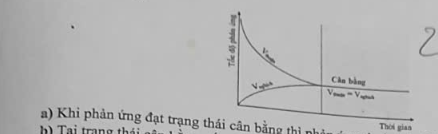
\includegraphics[width=0.45\textwidth]{images_crop/de104_do_thi_can_bang.png}
\end{center}
\choiceTF
{a) Khi phản ứng đạt trạng thái cân bằng thì phản ứng thuận và phản ứng nghịch dừng lại.}
{\True b) Tại trạng thái cân bằng, tốc độ phản ứng thuận bằng tốc độ phản ứng nghịch.}
{c) Đồ thị trên biểu diễn tốc độ của phản ứng một chiều phụ thuộc vào thời gian.}
{d) Khi phản ứng thuận nghịch xảy ra thì tốc độ phản ứng thuận tăng dần còn tốc độ phản ứng nghịch giảm dần.}
\loigiai{
a) Sai vì cân bằng hóa học là cân bằng động, phản ứng vẫn tiếp tục diễn ra.\\
b) Đúng vì tại cân bằng $v_{\text{thuận}} = v_{\text{nghịch}}$ (đường ngang trên đồ thị).\\
c) Sai vì đây là đồ thị của phản ứng thuận nghịch.\\
d) Sai vì ban đầu tốc độ thuận lớn nhất sau đó giảm dần, tốc độ nghịch bằng 0 sau đó tăng dần.}
\end{ex}

\bigskip
\noindent
\textbf{PHẦN III. Câu trắc nghiệm trả lời ngắn: (4 câu -- 1 điểm)}\\
\textit{Thí sinh trả lời từ câu 1 đến câu 4.}

\begin{ex}
Cho dung dịch $\ce{HNO3}$ tác dụng với các chất sau: $\ce{NH3}, \ce{CaCO3}, \ce{Ag}, \ce{NaOH}$. Có bao nhiêu phản ứng trong đó $\ce{HNO3}$ đóng vai trò acid theo Bronsted?
\shortans{3}
\loigiai{
Theo Brønsted, $\ce{HNO3}$ là acid khi nhường proton $\ce{H+}$:\\
- $\ce{NH3 + HNO3 -> NH4NO3}$ (nhường $\ce{H+}$ cho $\ce{NH3}$: là acid).\\
- $\ce{CaCO3 + 2HNO3 -> Ca(NO3)2 + CO2 ^ + H2O}$ (nhường $\ce{H+}$ cho $\ce{CO3^{2-}}$: là acid).\\
- $\ce{Ag + 2HNO3 -> AgNO3 + NO2 ^ + H2O}$ (phản ứng oxi hóa -- khử, $\ce{HNO3}$ là chất oxi hóa và môi trường).\\
- $\ce{NaOH + HNO3 -> NaNO3 + H2O}$ (nhường $\ce{H+}$ cho $\ce{OH-}$: là acid).\\
Vậy có 3 phản ứng: $\ce{NH3}, \ce{CaCO3}, \ce{NaOH}$.\\
\textbf{Đáp án: 3.}}
\end{ex}

\begin{ex}
Nhiệt phân các muối ammonium: $\ce{NH4Cl}, \ce{(NH4)2CO3}, \ce{NH4NO2}, \ce{NH4HCO3}, \ce{NH4NO3}$. Có bao nhiêu trường hợp thu được khí $\ce{NH3}$?
\shortans{3}
\loigiai{
- $\ce{NH4Cl ->[t^\circ] NH3 ^ + HCl ^}$ (có $\ce{NH3}$).\\
- $\ce{(NH4)2CO3 ->[t^\circ] 2NH3 ^ + CO2 ^ + H2O}$ (có $\ce{NH3}$).\\
- $\ce{NH4NO2 ->[t^\circ] N2 ^ + 2H2O}$ (không tạo $\ce{NH3}$).\\
- $\ce{NH4HCO3 ->[t^\circ] NH3 ^ + CO2 ^ + H2O}$ (có $\ce{NH3}$).\\
- $\ce{NH4NO3 ->[t^\circ] N2O ^ + 2H2O}$ (không tạo $\ce{NH3}$).\\
Có 3 trường hợp thu được $\ce{NH3}$: $\ce{NH4Cl}, \ce{(NH4)2CO3}, \ce{NH4HCO3}$.\\
\textbf{Đáp án: 3.}}
\end{ex}

\begin{ex}
Cho các chất (phân tử và ion): $\ce{NaOH}, \ce{H2S}, \ce{NH3}, \ce{CO3^{2-}}, \ce{S^{2-}}, \ce{NH4+}, \ce{PO4^{3-}}$. Theo quan điểm của Bronsted -- Lowry có bao nhiêu chất có thể là base?
\shortans{5}
\loigiai{
Theo Brønsted -- Lowry, base là chất nhận proton $\ce{H+}$:\\
- $\ce{NaOH}$ (chứa ion $\ce{OH-}$ nhận proton);\\
- $\ce{NH3}$ (nhận $\ce{H+}$ tạo $\ce{NH4+}$);\\
- $\ce{CO3^{2-}}$ (nhận $\ce{H+}$ tạo $\ce{HCO3-}$);\\
- $\ce{S^{2-}}$ (nhận $\ce{H+}$ tạo $\ce{HS-}$);\\
- $\ce{PO4^{3-}}$ (nhận $\ce{H+}$ tạo $\ce{HPO4^{2-}}$).\\
Vậy có 5 chất/ion là base: $\ce{NaOH}, \ce{NH3}, \ce{CO3^{2-}}, \ce{S^{2-}}, \ce{PO4^{3-}}$.\\
\textbf{Đáp án: 5.}}
\end{ex}

\begin{ex}
Cho cân bằng hóa học (trong bình kín) sau:
\[ \ce{N2(g) + 3H2(g) <=>[xt, t^\circ, p] 2NH3(g)} \quad \Delta_r H_{298}^\circ = -92\text{ kJ} \]
Trong các yếu tố: (1) Thêm một lượng $\ce{N2}$ hoặc $\ce{H2}$; (2) Thêm một lượng $\ce{NH3}$; (3) Tăng nhiệt độ của phản ứng; (4) Tăng áp suất của phản ứng; (5) Dùng thêm chất xúc tác. Có bao nhiêu yếu tố làm cho tỉ khối của hỗn hợp khí trong bình so với $\ce{H2}$ tăng lên?
\shortans{2}
\loigiai{
Tỉ khối so với $\ce{H2}$ tăng khi khối lượng mol trung bình $\overline{M}$ của hỗn hợp tăng:\\
- Yếu tố (4) Tăng áp suất làm cân bằng chuyển dịch theo chiều thuận (từ 4 mol khí tạo 2 mol khí), làm giảm số mol khí trong khi khối lượng bình không đổi $\implies \overline{M}$ tăng $\implies$ tỉ khối tăng.\\
- Yếu tố (2) Thêm $\ce{NH3}$ ($M = 17$) có khối lượng mol lớn hơn hỗn hợp ban đầu ($M_{\text{tb}} \approx 8{,}5$), làm tăng tỉ khối chung của hệ.\\
- Yếu tố (3) tăng nhiệt độ làm chuyển dịch chiều nghịch (giảm tỉ khối); (5) xúc tác không làm chuyển dịch cân bằng.\\
Vậy có 2 yếu tố làm tăng tỉ khối: (2) và (4).\\
\textbf{Đáp án: 2.}}
\end{ex}

\bigskip
\noindent
\textbf{PHẦN IV. TỰ LUẬN: (3 câu -- 3 điểm)}\\
\textit{Thí sinh trả lời từ câu 1 đến câu 3.}

\begin{ex}
\textbf{(1,0 điểm)} Viết biểu thức tính hằng số cân bằng ($K_C$) cho các phản ứng thuận nghịch sau:
\begin{enumerate}[(1)]
	\item $\ce{H2(g) + F2(g) <=> 2HF(g)}$
	\item $\ce{Fe2O3(s) + 3CO(g) <=> 2Fe(s) + 3CO2(g)}$
\end{enumerate}
\loigiai{
(1) Đối với phản ứng: $\ce{H2(g) + F2(g) <=> 2HF(g)}$
\[ K_C = \frac{[\ce{HF}]^2}{[\ce{H2}][\ce{F2}]} \]
(2) Đối với phản ứng: $\ce{Fe2O3(s) + 3CO(g) <=> 2Fe(s) + 3CO2(g)}$\\
Vì $\ce{Fe2O3}$ và $\ce{Fe}$ là chất rắn nguyên chất nên nồng độ của chúng không xuất hiện trong biểu thức $K_C$:
\[ K_C = \frac{[\ce{CO2}]^3}{[\ce{CO}]^3} \]}
\end{ex}

\begin{ex}
\textbf{(1,0 điểm)} Trộn lẫn $V\text{ mL}$ dung dịch $\ce{NaOH}\ 0{,}03\text{ M}$ với $V\text{ mL}$ dung dịch $\ce{HCl}\ 0{,}01\text{ M}$ được $2V\text{ mL}$ dung dịch Y. Dung dịch Y có pH là bao nhiêu?
\loigiai{
- Đổi thể tích: $V\text{ mL} = V \cdot 10^{-3}\text{ L}$.\\
- Số mol $\ce{OH-} = 0{,}03 \times V \cdot 10^{-3}\text{ mol}$; số mol $\ce{H+} = 0{,}01 \times V \cdot 10^{-3}\text{ mol}$.\\
- Phương trình phản ứng: $\ce{H+ + OH- -> H2O}$.\\
Vì $n_{\ce{OH-}} > n_{\ce{H+}}$ nên $\ce{OH-}$ dư sau phản ứng:\\
$n_{\ce{OH- dư}} = (0{,}03 - 0{,}01) \times V \cdot 10^{-3} = 0{,}02 \cdot 10^{-3}V\text{ mol}$.\\
- Tổng thể tích sau trộn: $V_Y = 2V\text{ mL} = 2V \cdot 10^{-3}\text{ L}$.\\
- Nồng độ ion $\ce{OH-}$ trong dung dịch Y:
\[ [\ce{OH-}] = \frac{0{,}02 \cdot 10^{-3}V}{2V \cdot 10^{-3}} = 0{,}01\text{ M} = 10^{-2}\text{ M}. \]
- $\text{pOH} = -\log[\ce{OH-}] = 2 \implies \text{pH} = 14 - \text{pOH} = 14 - 2 = 12$.\\
\textbf{Đáp số: $\text{pH} = 12$.}}
\end{ex}

\begin{ex}
\textbf{(1,0 điểm)} Nước cường toan trong tiếng Anh là Aqua Regia (nghĩa là nước hoàng gia) -- là hợp chất có tính ăn mòn mạnh, ở dạng lỏng, có màu vàng và dễ bay hơi, được sử dụng cho 1 số quy trình hóa học phân tích và để tinh chế vàng. Hãy nêu thành phần của nước cường toan và viết phản ứng của nước cường toan với vàng.
\loigiai{
- \textbf{Thành phần của nước cường toan (Aqua Regia):}\\
Là hỗn hợp gồm dung dịch $\ce{HNO3}$ đặc và dung dịch $\ce{HCl}$ đặc được trộn theo tỉ lệ thể tích:
\[ V_{\ce{HNO3}\text{ đặc}} : V_{\ce{HCl}\text{ đặc}} = 1 : 3 \]
- \textbf{Khả năng hòa tan vàng và phản ứng hóa học:}\\
Vàng ($\ce{Au}$) trơ về mặt hóa học, không tan trong $\ce{HNO3}$ đặc hoặc $\ce{HCl}$ đặc riêng rẽ, nhưng tan được trong nước cường toan do tính oxi hóa mạnh của $\ce{HNO3}$ kết hợp với ion $\ce{Cl-}$ tạo phức chất tan rất bền tetrachloroaurate(III):\\
\[ \ce{Au + HNO3 + 4HCl -> HAuCl4 + NO ^ + 2H2O} \]
\textit{(hoặc dạng ion: $\ce{Au + NO3- + 4Cl- + 4H+ -> [AuCl4]- + NO ^ + 2H2O}$)}.\\
Phức acid tetrachloroauric $\ce{HAuCl4}$ tan trong dung dịch, đồng thời giải phóng khí $\ce{NO}$.}
\end{ex}

\bigskip
\noindent
{\color{hfRed}\textbf{\large BẢNG TỔNG HỢP ĐÁP ÁN ĐỀ SỐ 104}}

\smallskip
\noindent
\textbf{1. PHẦN I (Trắc nghiệm nhiều phương án):}
\begin{center}
\begin{tabular}{|c|c|c|c|c|c|c|c|}
\hline
\textbf{1. B} & \textbf{2. C} & \textbf{3. A} & \textbf{4. A} & \textbf{5. A} & \textbf{6. C} & \textbf{7. D} & \textbf{8. D} \\ \hline
\textbf{9. D} & \textbf{10. C} & \textbf{11. D} & \textbf{12. C} & \textbf{13. B} & \textbf{14. D} & \textbf{15. C} & \textbf{16. D} \\ \hline
\end{tabular}
\end{center}

\noindent
\textbf{2. PHẦN II (Trắc nghiệm đúng sai):}
\begin{itemize}
	\item \textbf{Câu 1:} a) Đúng \quad|\quad b) Sai \quad|\quad c) Đúng \quad|\quad d) Đúng
	\item \textbf{Câu 2:} a) Sai \quad|\quad b) Đúng \quad|\quad c) Sai \quad|\quad d) Sai
\end{itemize}

\noindent
\textbf{3. PHẦN III (Trả lời ngắn):}
\begin{center}
\begin{tabular}{|c|c|c|c|}
\hline
\textbf{Câu 1} & \textbf{Câu 2} & \textbf{Câu 3} & \textbf{Câu 4} \\ \hline
3 & 3 & 5 & 2 \\ \hline
\end{tabular}
\end{center}

\begin{center}
\textbf{--------- HẾT ---------}\\
\textit{(Học sinh không sử dụng tài liệu và bảng tuần hoàn hoá học)}
\end{center}

\end{document}
